\section{Optimale løsning}
\label{sec:eksistens}
Hvis det lineære programmerings problem er konsistent, betyder det at der er en løsning til det, men bare fordi der er en løsning betyder det ikke at der er en optimal løsning.
Hvis der skal eksistere en optimal løsning må løsningsmængden ikke indeholde en linje.
\begin{defn}[Linje]
Lad $P\subseteq \mathds{R}^n $ være en polyede, da indeholder $P$ en \textbf{linje}, hvis $\vec{x}+\lambda\vec{d} \in P$ for alle $\lambda \in \mathds{R}_+$, hvor $\vec{x}\in P$ og $\vec{d} \in \mathds{R}^n$. Hvis $\vec{x}+\lambda\vec{d} \in P$ for $\lambda > 0$ eller $\lambda < 0$, siges $P$ at indeholde henholdsvis en positiv eller negativ halv linje.
\label{def:linje}
\end{defn}

\begin{defn} [Linje v2]
Lad $P\subseteq \mathds{R}^n $ være en polyede og $\vec{x} \in P$, da indeholder $P$ ikke en \textbf{Positiv halvlinje}, hvis $\forall \vec{d} \in \mathds{R}^n \nexists \lambda \in \mathds{R}_+ : \vec{x}+\lambda \vec{d} \in P$
\end{defn}
\\
Det betyder, at der til en løsning i polyeden kan lægges en retningsvektor til, denne retningsvektor bliver skaleret, så løsningen nu ligger et andet sted. Hvis der findes en retning, hvor der, selvom $\lambda$ er vilkårligt stor, resultere i at løsning stadig er i polyeden, så siges prolyede at have en linje.
%Det betyder, at der til en løsning kan lægges et vilkårligt stort multiplum af en vektor til, og summen vil stadig være en løsning, derfor må objektfunktionen nødvendigvis også kunne tage en vilkårlig stor værdi.
\begin{prop}
Lad løsningsmængden $\mathcal{F} = \{ \vec{x} \in \mathds{R}^n| A \vec{x} \geq b \} \subseteq \mathds{R}^n $  til det lineærer minimeringsproblem $\vec{c}^T\vec{x}$ indeholde en linje, da er løsningen $-\infty$.
\end{prop}
\begin{proof}
Da $\mathcal{F}$ indeholder en linje, følger det af Definition \ref{def:linje}, at der eksistere en vektor $\vec{x} \in \mathcal{F}$ og en vektor $\vec{d} \in \mathds{R}^n$, så $\vec{x}+\lambda \vec{d} \in \mathcal{F}$, for alle $\lambda \in \mathds{R}^n$. 
Derfor følger det at $\lambda$ kan vælges så $\vec{c}^T(\vec{x}+\lambda\vec{d}) = - \infty$, hvorfor løsningen må være $-\infty$.
\end{proof}
Bemærk, at da løsningsmængden indeholder en linje, kan løsningsmængden ikke være tom, er løsningsmængden tom, er problemet inkonsistent, og der eksistere derfor ikke en optimal løsning. 
Er løsningsmængden ikke tom, og uden linjer, da eksistere der en optimal løsning, som viser sig at være en mulig basisløsning.
\begin{stn}[Eksistens af optimal løsning]
Hvis løsningsmængden $\mathcal{F} =\{\vec{x} \in \mathds{R}^n| A \vec{x} \geq b \} \neq \emptyset$, til det lineære minimeringsproblem $\vec{c}^T\vec{x}$, ikke indeholder en linje, da vil der eksistere en optimal løsning $\vec{x^{**}}$, som er en mulig basisløsning.
\label{stn:eksistens}
\end{stn}
\begin{proof}
Antag, at $\vec{x} \in \mathcal{F}$ ikke er en mulig basisløsning, og lad $I =\{i | \vec{a_i}^T\vec{x}=b_i\}$ betegne indeksene for de lineært uafhængige aktive bibetingelser knyttet til løsningen $\vec{x}$.
Da $\vec{x}$ ikke er en mulig basisløsning, må $span(\{\vec{a_i}|i\in I\})$ være et ægte underrum til $\mathds{R}^n$, hvormed at der må eksistere en vektor $\vec{d} \in \mathds{R}^n$, så $\vec{a_i}^T\vec{d}=0$ for $i \in I$.
Da må $\vec{a_i}^T(\vec{x}\pm \vec{d})= \vec{a_i}^T\vec{x}=b_i$.
Vælg nu fortegn på $\vec{d}$ så $\vec{c}^T\vec{d}\leq 0$, da må $\vec{c}^T(\vec{x}+\lambda\vec{d}) \leq \vec{c}^T\vec{x}$ for en vilkårlig skalar $\lambda > 0$.
Da løsningsmængden ikke indeholder en linje, vil der være en øvre grænse for $\lambda$ før $\vec{x}+\lambda\vec{d} \notin \mathcal{F}$, svarende til $\lambda$et, der opfylder $\vec{a_j}^T(\vec{x}+\lambda\vec{d})=b_j$, hvor $\vec{a_j} \not in \{\vec{a_i}|i\in I\}$ er den første bibetingelse der bliver aktiv, se Figur \ref{fig:eksistens}.
Da $\vec{a_i}^T\vec{d}=0$ og $\vec{a_j}^T\vec{d} \neq 0$ medfører det at $\vec{a_i}$ og $\vec{a_j}$  er lineært uafhængige. 
Derfor kan $j$ tilføjes til $I$.
Gentag til at $|I|=n$.
\\ Antag nu, at $|I|=n$, derfor må $\vec{x}$ have $n$ aktive bibetingelser.
Da $\vec{x}\in \mathcal{F}$ medfører det, at $\vec{x}$ overholder alle ligheds bibetingelser, og at $\vec{x}$ er en mulig løsning. 
Derfor følger det af Definition \ref{def:basislosning}, at $\vec{x}$ er en mulig basisløsning.
\\Derfor må der fra en vilkårlig løsning $\vec{x}\in \mathcal{F}$ kunne konstrueres en mulig basisløsning $\vec{x^*}$ så $\vec{c}^T\vec{x^*} \leq \vec{c}^T \vec{x}$.
Dermed må den optimale løsning være den mulige basisløsning, der minimere objektfunktionen, hvorfor der eksistere en optimal løsning, som er en mulig basisløsning.
\end{proof}
\begin{figure}
\begin{center}
	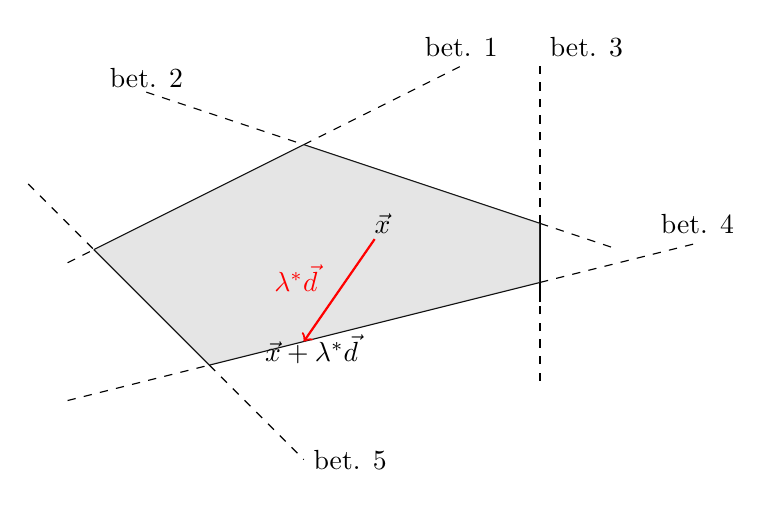
\begin{tikzpicture}[ latex
  s/.style={width=0}]

  %ligning 1
	\draw[domain=-1:-2/3,variable=\x,dashed] 	plot({\x},{0.5*\x+1});
	\draw[domain=-2/3:2,variable=\x] 			plot({\x},{0.5*\x+1});
	\draw[domain=2:4,variable=\x,dashed] 	plot({\x},{0.5*\x+1}) node[above] {bet. 1};
	
  %ligning 2
  	\draw[domain=0:2,variable=\x,dashed] 	plot({\x},{-(1/3)*\x+8/3}) node[above] at (0,2.6) {bet. 2} ;
	\draw[domain=2:5,variable=\x] 			plot({\x},{-(1/3)*\x+8/3});
	\draw[domain=5:6,variable=\x,dashed] 	plot({\x},{-(1/3)*\x+8/3});
	

  %ligning 3
  	\draw[domain=-1:0,variable=\y,dashed] 	plot({5},{\y});
	\draw[domain=0:1,variable=\y] 			plot({5},{\y});
	\draw[domain=1:3,variable=\y,dashed] 	plot({5},{\y}) node[above right] {bet. 3};
	
  %ligning 4
	\draw[domain=-1:4/5,variable=\x,dashed] 	plot({\x},{0.25*\x-1});
	\draw[domain=4/5:5,variable=\x] 			plot({\x},{0.25*\x-1});
	\draw[domain=5:7,variable=\x,dashed] 	plot({\x},{0.25*\x-1}) node[above] {bet. 4};
	
  %ligning 5
  	\draw[domain=-1.5:-2/3,variable=\x,dashed] 	plot({\x},{-\x}) ;
	\draw[domain=-2/3:4/5,variable=\x] 			plot({\x},{-\x});
	\draw[domain=4/5:2,variable=\x,dashed] 	plot({\x},{-\x}) node[right] {bet. 5} ;

  %løsningsmængden skraveret
	\fill[gray!80,nearly transparent] (4/5,-4/5) -- (-2/3,2/3) -- (2,2) -- (5,1) --(5,0.25) --  cycle;
	
  % vektor x
	\node[] (x) at (3,1) {$\vec{x}$};
	\draw[thick, color=red, ->](2.9,0.8) -- (2,-0.5) node[above, yshift=0.5 cm, xshift=-0.1 cm] {$\lambda^* \vec{d}$} ;
	\node[] (x) at (2.1, -0.6) {$\vec{x}+\lambda^* \vec{d}$};
 
\end{tikzpicture}
	\captionof{figure}{Der ligges et multiplum af en retnings vektor til vektor $\vec{x}$ til at summen gør betingelse $4$ aktiv.}
	\label{fig:eksistens}
\end{center}
\end{figure}
Det betyder at hvis det lineære programmerings problem er konsistent, da eksistere der enten en optimal løsning, blandt basisløsningerne eller den optimale løsning er $\pm \infty$.
Det kunne derfor være relevant at finde en måde, hvor den optimale løsning blandt basisløsningerne kan findes, her kan gøres brug af simplex metoden.



